%% This is file `DEMO-TUDaThesis.tex' version 4.03 (2025-04-02),
%% it is part of
%% TUDa-CI -- Corporate Design for TU Darmstadt
%% ----------------------------------------------------------------------------
%%
%% Copyright (C) 2018--2025 by Marei Peischl <marei@peitex.de>
%%
%% ============================================================================
%% This work may be distributed and/or modified under the
%% conditions of the LaTeX Project Public License, either version 1.3c
%% of this license or (at your option) any later version.
%% The latest version of this license is in
%% http://www.latex-project.org/lppl.txt
%% and version 1.3c or later is part of all distributions of LaTeX
%% version 2008/05/04 or later.
%%
%% This work has the LPPL maintenance status `maintained'.
%%
%% The current maintainer of this work is
%%   Marei Peischl <tuda-ci@peitex.de>
%%
%% The development repository can be found at
%% https://github.com/tudace/tuda_latex_templates
%% Please use the issue tracker for feedback!
%%
%% If you need a compiled version of this document, have a look at
%% http://mirror.ctan.org/macros/latex/contrib/tuda-ci/doc
%% or at the documentation directory of this package (if installed)
%% <path to your LaTeX distribution>/doc/latex/tuda-ci
%% ============================================================================
%%
% !TeX program = lualatex
%%

% Enable PDF/A via pdfmanagement and no longer via pdfx
\DocumentMetadata{
	pdfstandard=a-2b,
	pdfversion=1.7,% 2.0 is possible as well, but PDF/A-2b requires < 2.0
	lang=en,
}

\documentclass[
	german,% Main language as global option
	accentcolor=9c,% Choose accent color: For a list of available colors see the full tudapub documentation
	ruledheaders=section,% Section levels above this one will follow the ruled layout
	class=report,% Choose the base document class. Will choose the matching KOMA-Script class
	thesis={type=bachelor},% Thesis. For PhD thesis have a look at DEMO-TUDaPhd example file
	fontsize=11pt,% Basic font size. CI default setting of 9pt is too small for theses
	parskip=half-,% Use a parskip instead of indent, see KOMA-Script documentation
	custommargins=false,% Calculate margins using typearea
	marginpar=false,% Disable marginpar
	BCOR=5mm,% Binding correction
% 	accept-missing-logos=true,% No error in case logo files are not available
 	logofile=tools/logo-installation/TUDa-logos/tuda_logo.png,% In case logo should be replaced
]{tudapub}


%%%%%%%%%%%%%%%%%%%
% Language setup
%%%%%%%%%%%%%%%%%%%
\usepackage[english]{babel}
\usepackage{microtype}
\usepackage[autostyle]{csquotes}% \enquote, to simplify use of quotation marks

%%%%%%%%%%%%%%%%%%%
% Bibliography
%%%%%%%%%%%%%%%%%%%
\usepackage[sorting=none, citestyle=numeric-comp]{biblatex}
\addbibresource{ref.bib}% File name of BibTeX database

%%%%%%%%%%%%%%%%%%%
% Package suggestions for tables
%%%%%%%%%%%%%%%%%%%
\usepackage{array}% Fundamental tools for tables. Is automatically loaded by the following packages
%\usepackage{tabularx}% Tables with flexible columns to achieve fixed width
%\usepackage{longtable}% Tables across multiple pages
%\usepackage{xltabular}% Tables with fixed width spanning multiple pages
%\usepackage{booktabs}% Improved layout for horizontal rules in tables

%%%%%%%%%%%%%%%%%%%
% Package suggestions math
%%%%%%%%%%%%%%%%%%%
\usepackage{mathtools}% Extended version of amsmath
\usepackage{amssymb}% Additional symbols
\usepackage{siunitx}% Numbers and Units

\usepackage{subcaption}
\usepackage{tikz}
\usepackage{pgfplots}
\pgfplotsset{compat=1.18} % You can adjust the version as needed


\hypersetup{% Metadata adjustments, in case these are not set, the data provided for \maketitle will be used
	pdfauthor=Marei Peischl (peiTeX),
	pdfcreationdate=2024-05-03,
	pdfkeywords={TU Darmstadt; Corporate Design; LaTeX}
}

\title{Removal of undesired resonances of Terahertz antennas by inclusion of resistive feeds}
\author{Jakob Schmidt}
\reviewer{Prof. Dr. rer. nat. Sascha Preu \and Florian Bek M.Sc.}

% The following elements will be placed on the title page
\department{etit}% If defined the shorthand will be replaced by the full name otherwhise it's used directly.
\institute{Institute for Microwave Engineering and Photonics}
\group{Terahertz Devices and Systems}

\submissiondate{\today}
\examdate{\today}

%\tuprints{printid=XXXX,year=2022,license=cc-by-4.0}% License information for TUprints

\begin{document}

\maketitle

%% The affidavit was deactivated by default at the request of Department II.
%% According to the department, the legally binding text can be found at https://www.tu-darmstadt.de/studieren/studierende_tu/studienorganisation_und_tucan/hilfe_und_faq/artikel_details_de_en_37824.de.jsp
%%  The docx file should be used, printed out, signed, scanned and then integrated.
%% The easiest way to do this is to use the pdfpages package.
%%
%% For compatibility reasons for the other templates, the function is still available.
%% \affidavit[signature-image={\includegraphics[width=\width,height=1cm]{example-image}}, <there may be additional options here>]

\tableofcontents
% Additional lists like \listoffigures or acronyms might be added here
\listoffigures
\newpage

\chapter{Introduction}
In between the microwave and infrared (IR) frequencies of the electromagnetic (EM) spectrum lies Terahertz (THz) radiation (make ref to figure) \cite{zhangIntroductionTHzWave2010}. THz radiation refers to the frequency (wavelength) spectrum ranging from \num{100} \si{\giga\hertz} (\num{3} \si{\milli\meter}) up to \num{10} \si{\tera\hertz} (\num{30} \si{\micro\meter}). While microwave and infrared sources are able to provide high magnitudes of power at those frequencies, there has been a lack of efficient and feasible high power sources in the THz range \cite{perkowitzNavigatingTerahertzGap2020}. This has led to the common reference to the THz range as the \enquote{THz gap} (e.g. see \cite{dhillon2017TerahertzScience2017, williamsFillingTHzGap2006, zhangAdvancesTerahertzTechnology2021}). THz radiation shows potential in many fields. Thus tremendous efforts have been made in the last two decades to narrow the \enquote{THz gap}. Narrowing the gap has been achieved from both the microwave and the optical side. Advances have been made by extending the high frequency cut-off in purely electronic RF devices, decreasing the lower cut-off frequencies of purely optical IR devices or even by combining the two approaches \cite{preuTunableContinuouswaveTerahertz2011}. Progress has been made not only driven by advances in THz technology but also a wide range of applications. One of the most important techniques using THz radiation is THz Time Domain Spectroscopy (THz-TDS). In many fields such as pharmaceutics \cite{huangProgressApplicationTerahertz2023}, materials sciences \cite{zhangApplicationTHzTDSCharacterization2024}, chemistry \cite{fischerChemicalRecognitionTerahertz2005} and many more (e.g. see \cite{petrovMobileNearfieldTerahertz2023, markelzPerspectiveTerahertzApplications2022,TerahertzSpectroscopyIts2011,kleine-ostmannReviewTerahertzCommunications2011}), THz-TDS has proven to be a valuable technique.

The THz frequency range exhibits several significant spectral features, including rotational transitions of gas-phase molecules, large-amplitude vibrational modes of organic compounds, lattice vibrations in solids, energy gaps in superconductors and intraband transitions in semiconductors \cite{PrinciplesTerahertzScience2009}. Techniques like THz-TDS exploit these characteristic material responses to probe and analyze the interaction of THz radiation with matter. Compared to the neighboring radio and infrared regions, the THz band exhibits much higher atmospheric opacity due to molecular rotational absorption lines \cite{fedorovPowerfulTerahertzWaves2020}. Water vapor plays a dominant role in attenuating THz radiation as it strongly absorbs energy in this frequency range. The unique spectral line structures of different molecular species allow for their identification within unknown samples. The shapes of these lines offer valuable insight into microscopic processes such as molecular collisions \cite{PrinciplesTerahertzScience2009}.

Since being introduced THz-TDS has been applied to many materials. Those include biomolecules, medicines, cancer tissue, DNA, proteins and bacteria \cite{chenLargeOxidationDependence2005,waltherNoncovalentIntermolecularForces2003,fischerTerahertzTimedomainSpectroscopy2005}. Here, THz-TDS can deliver valuable information IR spectroscopy cannot. One example is the ability to observe intermolecular vibrations in chemicals and organic molecules where the intramolecular mode appears in the IR region \cite{nagaiDirectEvidenceIntermolecular2005}. Intermolecular vibration studies using THz-TDS are expected to enhance our knowledge of larger biomolecules and the human body \cite{tonouchiCuttingedgeTerahertzTechnology2007}. 

Because of the low photon energy (typically $\sim 1-10$ \si{\milli \electronvolt}) \cite{yangBiomedicalApplicationsTerahertz2016}, THz radiation does not ionize molecules. This makes THz-tomography a great alternative to conventional X-ray techniques, which can break down molecules. THz-TDS can be combined with density functional theory \cite{chenCombinationTerahertzSpectroscopy2022} to study amino acids \cite{liaoAminoacidClassificationBased2023}, peptides \cite{neuTerahertzSpectroscopyTetrameric2019}, drugs \cite{kawaseNondestructiveTerahertzImaging2003} and explosives \cite{daviesTerahertzSpectroscopyExplosives2008}. THz radiation is transparent to most dry dielectric materials due to its relatively long wavelength. THz waves easily penetrate most clothing \cite{prokschaTerahertzInsightsFabric2024} or packaging \cite{wietzkeTerahertzSpectroscopyPolymers2011} material. This makes THz-TDS a valuable technique in security applications, quality and process controls and nondestructive analysis of materials and devices. THz radiations sensitivity to water can be used to control food and agricultural products \cite{afsah-hejriTerahertzSpectroscopyImaging2020}. For example, damage to fruits can be evaluated and the water content in vegetables can be monitored. Within the industrial food sector, compact and high-speed THz cameras capable of providing instant quality control information of products on conveyer belts are needed \cite{THzSecurityApplications}. 

Examining metamaterials is a subject of great interest as they enable engineered electromagnetic properties not found in naturally occurring materials \cite{lakamanahalliMetamaterialsComprehensiveReview2024}. Metamaterials can exhibit singular electromagnetic properties like a negative refraction index, an effect not found in nature \cite{ramakrishnaPhysicsApplicationsNegative2008}. As THz-TDS provides both amplitude and phase information it can be crucial for understanding the electromagnetic properties and engineering of metamaterials \cite{rouxPrinciplesApplicationsTHz2014}. 

\begin{figure}[!btp]
    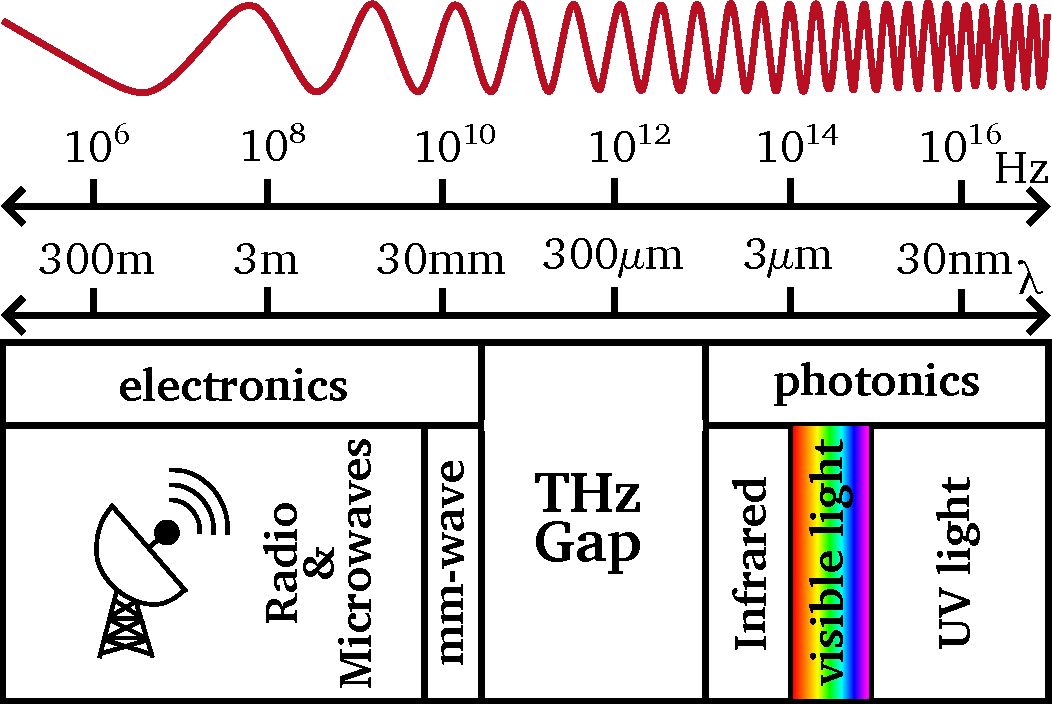
\includegraphics[height=0.4\textwidth]{figures/THz_overview.pdf}
    \centering
    \caption{Schematic diagram depicting the location of the so called THz gap in between electronically and optically generated frequencies.}
    \label{thz_overview}
\end{figure}










\section{Motivation}

\section{Objective and Thesis Outline}
The objective of this thesis is to reduce low frequency resonances in H-Dipole PCAs when being used in pulsed operation THz systems. These resonances limit the bandwidth of a measured signals Fourier Transform and are thus a major problem in broadband apllications. Adding NiCr sections to our antenna feeds we hope to limit low frequency surface current resonances. Multiple configurations of the NiCr-induced feeds are first investigated in CST simulations before the antennas are fabricated ans investigated concerning their THz performace as photoconductive THz sources.  

Chapter 2 presents the theory needed for understanding THz-TDS and its challenges. Photoconductor theory, especially the principles of photomixing for pulsed operation and suitable antenna geometries for THz-TDS are presented. The cause for low frequency surface current resonances and their effects on THz-TDS are explained. Chapter 3 deals with designing and simulating an antenna that fulfills our needs. Suitable antenna topologies combined with NiCr-induced feeds are presented and simulated in CST Studio Suite. The simulation results are presented. Chapter 4 presents the fabrication process of the antennas to be investigated. The devices are also characterized in terms of their dark current (DC) IV-characteristics. Chapter 5 explains the TDS measurement setup, the steps taken for alignment and how the measurement data is to be analyzed. In chapter 6, the THz performance of the devices is investigated. We present the time domain and frequency domain signals and compare the effects of NiCr-induced feeds, as well as comparing the results to our simulations. Chapter 7 summarizes and concludes the work. An outlook on possible future work is given.  

\chapter{Theory}

\section{THz Time Domain Spectroscopy}
Spectroscopy measures absorbtion and emission of light and other radiation by matter \cite{atascientificUnderstandingSpectrometrySpectroscopy2020}. The energy, wavelength, or frequency of photons that pass through a sample is detected that way. In the particular case of THz-TDS, matter is probed with very short Thz pulses.
The pulse usually has a duration of a few picoseconds \cite{neuTutorialIntroductionTerahertz2018}. The THz time domain signal measures the trasient electrical field. This is a major advantage of THz-TDS because intensity and phase of the electrical field are measured simultaneously \cite{zhaoPrincipleTerahertzTimeDomain2023}.

A conventional THz-TDS system consists of a femtosecond laser, a terahertz source, mirrors for beam steering, delay stages, optical beam splitters, focusing and collimating optics such as parabolic mirrors, and a detector. The basic working principle is described in the following, mainly as a review of \cite{neuTutorialIntroductionTerahertz2018,PrinciplesTerahertzScience2009}. More detailed explanations are given in Chapter 5.


In a pulsed THz-TDS system, an unltrafast laser is used to drive both the THz detector and source. As the electrical field of the THz signal usually has a time duration of a few picoseconds, optical detection techniques with sub-picosecond resolution are needed. The laser's pulse duration lies in the $\sim$ \num{100} \si{\femto\s} range. This ultrashort NIR optical pulse is beamsplit along two paths to generate and detect the timedependent THz field. 

One of the beams goes through a translational stage to provide a relative time delay. The time delay ensures that we can measure the amplitude of the electrical field at the detector at multiple points in time. The temporal delay is achieved by increasing the path length the beam. The travel time of a laser pulse is $t = s/c$, where $s$ is the path length and $c$ is the speed of light. 

The other beam is used as an optical pump, illuminating the THz emitter to generate the THz signal. The signal is focused onto a THz detector. Here, the electrical field of the THz signal is measured by using the delayed beam as probing pulses. The THz field is measured in the time-domain. THz-TDS makes use of the convolution of the short probing pulse with the longer THz signal. The instantaneous signal at the detector can be described as 

\begin{equation}
	S(t) \propto I_{opt}(t)\cdot E_{THz}(t),
\end{equation}

with $I_{opt}(t)$ being the optical intensity of the probing pulse and $E_{THz}(t)$ being the Thz field at the detector interface. This signal must be detected with subpicosecond resolution. All existing detectors are too slow, so the convolution of the two pulses is measured instead: 

\begin{equation}
	S(t) \propto I_{opt}(t) \ast E_{THz}(t).
\end{equation}

The duration of the optical pulse is significantly shorter than the duration of the THz signal. We can approximate it as an ideal pulse, hence the delta-function $\delta(t)$, yielding in

\begin{equation}
	S(t) \propto I_{opt}(t) \ast E_{THz}(t) \approx \delta(t) \ast E_{THz}(t) = E_{THz(t)}.
\end{equation}

Because of the convolution, the THz detector is only sensitive when both signals arrive at the same time. The probing pulse being approximated as the delta-function allows us to measure the amplitude and phase of the THz signal as a function of time. With knowledge about the amplitude and the phase, not only the absorption but also the dispersion of the sample can be obtained by analyzing the Fourier transforms of the waveforms. 

\textbf{TODO: Abbildung von THz Puls und Fourier Transformierter}

\section{THz Emitters based on Photocondcutive Antennas}
% Two distinct methods exist for THz generation and detection using ultrafast quantum cascade laser systems. THz radiation can be generated or detected by making use of non-linear optics. Non-linear optics exploit crystals with large second-order non-linear susceptibilities \cite{THzSourcesDetectors, kimHighlyNonlinearOptical2021} for THz generation or detection. By using a photoconductive material and utilizing the concept of photomixing, THz waves can also be generated or detected. This thesis will only focus on the photoconductive approach. 

PCAs are among the most established devices for generating and detecting THz radiation. They operate as ultrafast optical switches. When a laser pulse illuminates the photoconductor, its conductivity increases abruptly due to the generation of electron-hole pairs. A bias voltage applied across the electrodes accelerates these carriers, producing a photocurrent that drives THz radiation in the antenna structure.  

Efficient THz emission requires sub-picosecond switching. The switch-on time is governed by the excitation laser pulse duration, while the switch-off time is limited by the carrier lifetime of the semiconductor material. Suitable PCA substrates must therefore combine short carrier lifetimes with high carrier mobility and high breakdown voltage to ensure both ultrafast response and robust operation.  

A PCA consists of a small active photoconductive region between metallic electrodes. The electrodes provide the bias field and couple the transient photocurrent into free-space radiation. The underlying physical mechanisms and corresponding mathematical description are discussed in the following sections.



% PCAs are one of the most established for generating and detecting THz radiation. A PCA is a semiconductor device that acts as an optical switch by increasing its conductivity when illuminated. The semiconductor device (photoconductor) features a direct band-gap. Photoconductors are operated with lasers and are based on the principle of photomixing \cite{peytavitTHzPhotomixers2021}. Two interfering laser beams forming an optical beat signal are focused on the photoconductor. When the beat signal's energy level is higher than that of the semiconductor's band-gap energy, free electron-hole pairs are photo-generated. A bias voltage applied to the electrodes of the antenna separates the carriers to create a displacement current. The current oscillates with the envelope of the absorbed laser light, resulting in a THz signal \cite{nandiErAsInAlGaAsPhotoconductors2021}. To emit or detect THz radiation, the switching in a PCA must happen within a subpicosecond timescale. The switch-on time depends on the duration of the laser pulse. The switch-off time is mainly determined by the lifetime of photoexcited carriers in the semiconductor. Both a short laser pulse and a short carrier lifetime are essential for ultrafast switching. High carrier mobility and high breakdown voltage are also important for achieving good material performance. PCAs usually consist of a photomixing device, often called active region, sitting in between the antenna's electrodes. The electrodes help emit or detect the THz signal. The mathematics for THz generation through photomixing are given in the following sections. 

\subsection{Principles of Photomixing for Pulsed Operation}
To explain the principles of pulsed operation for THz-TDS, continuos wave (CW) operation (see Figure \ref{fig:cw_basics}) is explained beforehand. The principles of pulsed operation are then derived from CW operation. This section is mainly a review of \cite{nandiErAsInAlGaAsPhotoconductors2021,faridiPulsedFreeSpace2023,preuPrinciplesTHzGeneration2015}.

\begin{figure}
	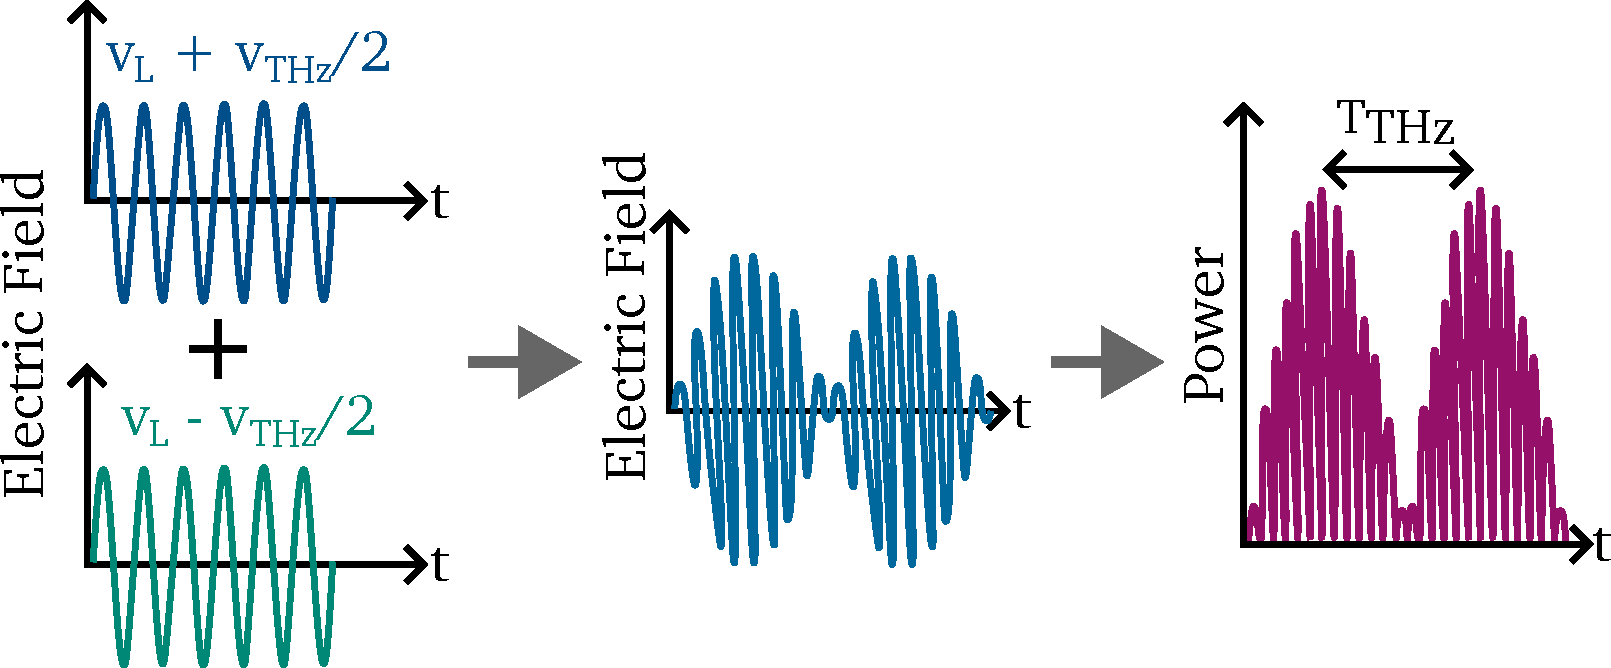
\includegraphics[width=0.85\linewidth]{figures/cw_principles.pdf}
	\centering
	\caption{Basic working principle of the continuos wave photomixing process. Two laser signals are heterodyned. The resulting power modulation shows a beat node at the difference frequency $\nu_{THz} = 1/T_{THz}$ of the two signals.}
	\label{fig:cw_basics}
\end{figure}

\subsubsection{CW operation}
In CW photomixing, two single-mode lasers operate at a difference frequency $\omega_L = \omega_0 \pm \omega_{THz}$. The two laser signals are heterodyned, producing an intensity beat at the difference frequency of the two lasers. The photoconductor is illuminated by the heterodyned laser signal. If the modulation of the lasers exceeds the semiconductor band-gap energy, charge carriers are generated at the beat frequency. The heterodyned signal illuminating the photoconductor is given by 
% CW THz radiation is generated using two CW lasers. The lasers have a difference frequency of $\omega_L = \omega_0 \pm \omega_{THz}$. The photon energy of the lasers has to be higher than the band-gap energy of the photoconducting material: $h\nu_L > E_G$, 
% where $\nu_L = \omega_L / 2\pi$, $h$ is Planck’s constant and $E_G$ is the bandgap energy of the material. The two laser signals are heterodyned. Heterodyning means mixing two signal's frequencies to achieve a resulting signal frequency that is shifted into another frequency range. A fiber coupler is used for feeding the heterodyned signal into the photoconductor with an optical field of

\begin{equation}
	\vec{E}(t) = \vec{E}_1(t) + \vec{E}_2(t) = \vec{E}_{1,0}e^{i(\omega_L - \omega_{THz}/2)t} + \vec{E}_{2,0}e^{i(\omega_L + \omega_{THz}/2)t - i\phi},
\end{equation}
where $\phi$ is the phase difference of the laser signals. The optical intensity of the absorbed laser power is given by 
\begin{equation}
	I_L(t) \sim |\vec{E}(t)|^2 = |\vec{E}_{1,0}(t)|^2 + |\vec{E}_{2,0}(t)|^2 + 2|\vec{E}_{1,0}(t) \cdot \vec{E}_{2,0}(t)|\cos(\omega_{THz}t + \phi), 
\end{equation}

which can be rewritten in terms of laser power as 

\begin{equation}
	P_L(t) = P_1 + P_2 + 2\sqrt{P_1 P_2}\cos(\beta)\cos(\omega_{THz}t + \phi), 
\end{equation}

where $\beta$ is the angle between the polarization of the electric fields. In an ideal photoconductor, all laser light is absorbed. This yields an ideal photocurrent 
\begin{equation}
	I_{Ph}^{Id}(t) = \frac{eP_L(t)}{h\nu_L} = \frac{e(P_1+P_2)}{h\nu_L} + 2\frac{e\sqrt{P_1P_2}}{h\nu_L}\cos(\beta)\cdot\cos(\omega_{THz}t + \phi),
	\label{eq_iph}
\end{equation}

where $e$ denotes the elementary charge.
We see that the ideal photocurrent $I_{Ph}^{Id}(t)$ consists of a DC component $I_{DC}^{Id}$ and an AC component $I_{THz}^{Id}(t)$.
The DC component is given by 
\begin{equation}
	I_{DC}^{Id} = \frac{e(P_1+P_2)}{h\nu_L}.
\end{equation} 
The AC component of the ideal photocurrent is given by the expression
\begin{equation}
	I_{THz}^{Id}(t) = 2\frac{e\sqrt{P_1P_2}}{h\nu_L}\cos(\beta)\cdot\cos(\omega_{THz}t + \phi).
\end{equation}

To maximize the THz output, the AC part of the photocurrent has to be maximized. We see that $I_{THz}^{Id}$ is at its maximum when $P_1 = P_2 = P_L = P_{tot} / 2$ and $\beta = 0$. This is equivalent to identical power and polarization of the two laser signals. With these assumptions the amplitude of the ideal photocurrent's THz part becomes $I_{THz}^{Id} = eP_{tot} / (h\nu) = I_{DC}^{Id} = I^{Id}$. Ultimately inserting our assumptions into \ref{eq_iph} we get 
\begin{equation}
	I_{Ph}^{Id} = I^{Id}[1 + \cos(\omega_{THz}t + \phi)].
	\label{eq8}
\end{equation}

The generated photocurrent is fed into a radiating element, usually an antenna. This antenna is fabricated on the same semiconducting material as the photomixing device. The antenna shows a radiation resistance $R_A$, yielding the ideal emitted THz power 
\begin{equation}
	P_{THz}^{Id}=\frac{1}{2}R_A (I_{THz}^{Id})^2.
	\label{eq_thz_pow}
\end{equation}

\subsubsection{Pulsed Operation}

In pulsed operation, the semiconductor absorbs a short optical pulse. The photocurrent generated by this pulse results in THz radiation when fed into a radiating element like an antenna. The emitted THz field is proportional to the time derivative of the photocurrent generated by the lasers \cite{preuTunableContinuouswaveTerahertz2011}
\begin{equation}
	E_{THz} \propto \frac{\partial I_{Ph}(t)}{\partial t}.
\label{eq1}
\end{equation}

The CW generation of THz radiation can be extended to the pulsed approach. Under pulsed operation, multiple laser frequencies are mixed to form a single laser pulse denoted by 
\begin{equation}
	\vec{E}(t) = \sum_j^n \vec{E}_je^{i(\omega_j t + \phi j)}.
\label{eq3}
\end{equation}
Here, $\omega_j = 2 \pi \nu_j$ are the angular frequency components of each electrical field $\vec{E}_j$ and $\phi_j$ are the corresponding phase components. Assuming a typical mode locked femtosecond laser we get the following properties: 
\renewcommand{\labelenumi}{\alph{enumi})}
\begin{enumerate}
	\item The frequency components are equally spaced in the spectral domain: $\nu_j - \nu_{j-1} = R_p$, where $R_p$ is the repetition rate of the laser.
	\item The phase has a fixed, linear relationship: $\phi_j - \phi_{j-1} = const.$
\end{enumerate}

The mode locking allows for very short laser pulses in the femtosecond range.

To obtain the ideal frequency spectrum of the emitted THz field, the signal has to be Fourier transformed. Fourier transforming eq. \eqref{eq1} yields

\begin{equation}
	E_{THz}(\omega) \propto \mathcal{F}\left\{ \frac{\partial I_{Ph}(t)}{\partial t} \right\} = i\omega I_{Ph}(t), 
\end{equation}

where $\mathcal{F}\{\cdot \}$ denotes the Fourier transform and $I_{Ph}(\omega)$ is the spectrum of the photocurrent. Ideally, the spectrum of the photocurrent is proportional to the spectral width of the photocurrent. Note that the spectral width $\Delta \omega$ is inversely proportional to the temporal width $\Delta \tau$, resulting in $\Delta \omega \Delta \tau = 0.5$ The optical pulse duration must be shorter than the period of the maximum THz frequency to be obtained. 

Deriving the emitted THz spectrum under pulsed operation is fairly complex and would be beyond the scope of this thesis. Detailed derivations can be found in \cite{preuPrinciplesTHzGeneration2015}. In the following, only some fundamental steps in obtaining the emitted THz field are given. From eq. \eqref{eq1} we know that the field generated by a radiating structure like an antenna is proportional to the time-derivative of the current. We also know that the ideal photocurrent is proportional to the total optical power. Assuming a laser beam that shows Gaussian distributed intensity, meaning $\vec{E}_j$ is Gaussian distributed, eq. \eqref{eq3} becomes
\begin{equation}
	\vec{E}(t) = \vec{A}(t)e^{i\omega_Lt}.
\label{eq4} 
\end{equation}

$\vec{A}(t)$ denotes the complex envelope of the pulse while $\omega_L$ is the laser pulses central frequency. With the mode-locked laser property of a linear phase relationship, the pulse is Fourier transform-limited (bandwidth-limited), yielding an envelope of
\begin{equation}
	\vec{A}(t) = \vec{A}_0 e^{\frac{-t^2}{\tau^2}},
\end{equation}

with $\tau$ being the time-domain $1/e^2$ width. The  $1/e^2$ width is the difference of the two points in the Gaussian beam where the intensity falls to $1/e^2 = 0.135$. 

The Gaussian pulse's optical intensity is once again given by
\begin{equation}
	I_L(t) \sim |\vec{E}_L(t)|^2 = I_{L,0}e^{\frac{-2t^2}{\tau ^2}}.
\end{equation} 

Note that $I_{L,0} \sim |\vec{A}_0|^2$ which corresponds to the peak intensity of the beam. 
Fourier transforming eq. \eqref{eq4} gives us the spectral components of the pulse:

\begin{equation}
	V(\nu) =  \mathcal{F}\left\{\vec{A}(t)e^{i\omega_Lt} \right\}
	= \int_{-\infty}^{+\infty}E_L(t)e^{-i2\pi\nu t}dt = |V(\nu)|e^{i\psi(\nu)}.
\end{equation}

$\psi(\nu)$ denotes the spectral phase in this case. For a Gaussian beam, the spectral intensity is given by:
\begin{equation}
	S_I(\nu) = |V(\nu)|^2 \sim \exp[-2\pi^2\tau^2(\nu - \nu_L)^2]. 
\end{equation}

The spectral $1/e^2$ width here is described by $\sigma$, with $\tau = \sqrt{2}/(\pi \sigma)$. We already know from eq. \eqref{eq_iph} that the photocurrent is proportional to the laser power, $I_{Ph}(t) \sim P_L(t)$. Thus the ideal generated photocurrent can be expressed as 

\begin{equation}
	I_{Ph}^{Id}(t) = \frac{eP_L(t)}{h\nu_L} = \hat{I}_{L,0} e^{\frac{-2t^2}{\tau^2}},
\label{eq_gauss}
\end{equation}

where $\hat{I}_{L,0}$ is the maximum generated photocurrent. From eq. \eqref{eq_gauss} we can conclude that in an ideal case, the resulting photocurrent is Gaussian distributed because the carriers respond to the lasers envelope. 

\subsection{Principles of THz Detection by Photomixing for Pulsed Operation}

Photoconductors can also act as THz detectors, based on the same mechanisms as generation. Implementing PCA based THz detectors is explained in the following as a review of \cite{preuPrinciplesTHzGeneration2015,castro-camusPhotoconductiveResponseCorrection2008}. An ultrafast laser pulse and a THz transient are focused onto the active region between the antenna electrodes. The laser pulse generates electron–hole pairs. The incident THz field provides the bias, modulating charge-carrier motion. Since both signals overlap in space and time, the photocurrent is given by the convolution of the optical pulse with the THz field. The photocurrent is heavily dependent on the incident THz field and the conductivity of the semiconducting material. The latter defines the mode of operation in THz detection. Photoconductive detectors work in direct sampling or integrating mode. They can also be configured to be used in intermediate sampling modes, depending on the semiconducting properties.

% An ultrafast laser pulse and a THz signal generated by the same laser signal are focused onto the active region in between the antenna electrodes. The optical pulse of the laser creates free electron-hole pairs that can be converted into a current by applying a bias field. This bias field is provided by the incoming THz signal. The electrical field of the THz signal controls the current flow. As the laser signal and the incoming THz signal incite the active region simultaneously, the photocurrent is given by convolution of the two signals. The generated DC current is heavily dependent on the incoming THz field and the conductivity of the semiconducting material. The latter defines the mode of operation in THz detection. Photoconductive detectors work in direct sampling or integrating mode. They can also be configured to be used in intermediate sampling modes, depending on the semiconducting properties.

\subsubsection{Direct Sampling}

In materials with ultrashort carrier lifetimes ($\tau_c \ll 1$\,\si{\pico \s}), charge-carriers recombine almost immediately. This produces a delta-like conductivity spike, only lasting as long as the device is illuminated. The photocurrent thus samples the instantaneous THz field:
\begin{equation}
    I(\tau) \propto E_{THz}(t=\tau).
\end{equation}
By varying the temporal overlap $\tau$ between laser and THz pulse, the transient field can be reconstructed.

% Direct sampling detectors work by exploiting the properties of highly resistive semiconducting materials which exhibit very low charge-carrier lifetimes $\tau_c \ll 1$ \si{\pico \s}. The optically generated charge-carriers are trapped very quickly by scattering and trapping centers in the semiconductor's crystal structure. The generated electron-hole pairs provide a conductivity spike which only lasts as long as the device is illuminated by the laser pulse. In an ideal case, the conductivity spike can be modeled as a delta function. As the generated photocurrent is given by the convolution of the laser pulse and the incoming THz radiation, in this case, it only samples the point of the THz signal that overlaps spatially and temporally with the laser pulse. This means that the incoming THz transient can be reconstructed by changing the temporal overlap $\tau$ between the laser pulse and the THz wave. Assuming the spike in conductivity to be much shorter than the THz signal's transient features, the THz wave is given by

% \begin{equation}
% 	I(\tau) \propto E_{THz}(t=\tau).
% \end{equation}

\subsubsection{Integrating Detection}
For long carrier lifetimes ($\tau_c > 1$\,\si{\pico \s}), the photoconductor remains conductive well beyond the duration of the THz transient. The photocurrent is given by the integral over the convolution of the transient electrical field and the material conductivity $\sigma(t)$:
\begin{equation}
    I(\tau) \propto \int_{-\infty}^{+\infty} E_{THz}(t)\sigma(t=\tau)\, dt .
    \label{eq_conv_integration_detection}
\end{equation}
Assuming a step-like conductivity, this reduces to
\begin{equation}
    I(\tau) \propto \int_{\tau}^{+\infty} E_{THz}(t)\, dt.
    \label{eq_conv_int_det_2}
\end{equation}
The THz field can be reconstructed by differentiating the detected photocurrent with respect to time. Long-lifetime devices enable high bandwidth (limited by the laser pulse duration) but also integrate noise, ultimately lowering SNR. In practice, optimal detection combines aspects of direct and integrating operation.

\subsubsection{Intermediate Case and Deconvolution}

For carrier lifetimes comparable to the THz pulse duration, the photocurrent cannot be directly related to $E_{THz}(t)$ by proportionality or differentiation. Instead, a convolution approach is used \cite{castro-camusPhotoconductiveResponseCorrection2008}:
\begin{equation}
    I(\tau) \propto \beta \int_{-\infty}^{+\infty} E_{THz}(t)\Phi(t-\tau)\, dt ,
    \qquad \beta \propto P_L T_{12} \lambda ,
    \label{eq_conv_integration_detection_2}
\end{equation}
with $\Phi(t) = \theta(t)e^{-t/\tau_{rec}}$ the normalized conductivity response and $T_{12}$ the Fresnel transformation coefficient. Fourier transforming yields
\begin{equation}
    I(\omega) = \beta E_{THz}(\omega)\Phi(\omega).
    \label{eq_FFT_int_det}
\end{equation}
The THz field follows by inverse transform:
\begin{equation}
    E_{THz}(t) = \frac{1}{\beta} \mathcal{F}^{-1}\left\{\frac{I(\omega)}{\Phi(\omega)}\right\}
    = \frac{1}{\beta} \mathcal{F}^{-1}\left\{I(\omega)\left(\tfrac{1}{\tau_c}+i\omega\right)\right\}.
\end{equation}
Thus, knowing $\tau_{rec}$ suffices to reconstruct $E_{THz}(t)$ numerically. In this work, the NiCr-modified PCAs are used exclusively as receiving antennas. Knowledge about detection principles is valuable for analyzing and interpreting measurements. 

% Integrating detection occurs in semiconductors with long charge-carrier lifetimes $\tau_c > 1$ \si{\pico \s}. The carrier lifetime significantly exceeds the duration of the incoming THz transient. As a result, the photoconductive material remains excited well beyond the duration of the THz pulse. The generated photocurrent is ultimately given by the integral over time of the convolution of the transient electrical field and the material conductivity $\sigma(t)$:

% \begin{equation}
% 	I(\tau) \propto \int_{-\infty}^{+\infty} E_{THz}(t)\sigma(t = \tau)dt.
% 	\label{eq_conv_integration_detection}
% \end{equation}

% The optically generated current samples the electrical field. 
% By deconvolution of Eq. \ref{eq_conv_integration_detection}, the actual THz field can be obtained, assuming $\sigma(t)$ is known. Assuming $\sigma(t)$ to rise like a step function upon photoexcitation, Eq. \ref{eq_conv_integration_detection} becomes 

% \begin{equation}
% 	I(\tau) \propto  \int_{\tau}^{+\infty} E_{THz}(t)dt.
% 	\label{eq_conv_int_det_2}
% \end{equation}

% The THz field can be reconstructed by differentiating the detected photocurrent with respect to time. Eq. \ref{eq_conv_integration_detection} shows that high bandwidth detectors can be fabricated with long carrier lifetime materials. Bandwidth is rather limited by the rise time of the photoconductivity, which is mainly dependent on the duration of the laser pulse. However, for long carrier lifetimes we also integrate over noise as long as the semiconductor is still photoconductive, reducing the overall SNR. A best practice approach for THz pulse detection is to combine direct sampling and integrating detection to achieve high bandwidth with high SNR. 

% PCAs which produce the highest SNRs usually have photoconductive lifetimes similar to the duration of a THz transient. The THz field of the sampled photocurrent of such devices however cannot be directly translated via proportionality or differentiation. Thus, a numerical deconvolution approach is proposed in \cite{castro-camusPhotoconductiveResponseCorrection2008}. We can rewrite eq. \ref{eq_conv_int_det_2} as 

% \begin{equation}
% 		I(\tau) \propto \beta \int_{-\infty}^{+\infty} E_{THz}(t)\Phi(t - \tau)dt,
% 		\qquad \beta \propto P_L T_{12} \lambda
% 	\label{eq_conv_integration_detection_2}
% \end{equation}

% where $\beta$ is a constant dependent on the Fresnel transformation coefficient $T_{12}$ for light from a laser gate beam of center wavelength $\lambda$ and average laser power reaching the semiconductor surface $P_L$. $\Phi(t)$ is the normalized time dependent conductivity which can be expressed by 

% \begin{equation}
% 	\Phi(t) = \theta(t)e^{-t/\tau_{rec}},
% \end{equation}

% where $\theta(t)$ describes a step function. In most THz-TDS systems, the duration of the laser pulse is much shorter than the duration of the THz transient to be measured and the pulse can be approximated as a delta function. Only then does the step-function assumption hold. As the generated photocurrent is a measure of the electrical field of the incoming THz signal, Fourier-transforming $I(\tau)$ yields the spectrum of the THz transient

% \begin{equation}
% 	I(\omega) = \beta E_{THz}(\omega) \Phi(\omega). 
% 	\label{eq_FFT_int_det}
% \end{equation}

% The time-domain signal of the electrical field is then given by taking the inverse Fourier-transformation of Eq. \ref{eq_FFT_int_det}
% \begin{equation}
% 	E_{THz}(t) = \frac{1}{\beta} \mathcal{F}^{-1}\left\{\frac{I(\omega)}{\Phi(\omega)} \right\} =  \frac{1}{\beta} \mathcal{F}^{-1} \left\{I(\omega)(\frac{1}{\tau_c} + i \omega)
% 	 \right\}.
% \end{equation}

% This deconvolution approach provides an efficient way of extracting the detected THz-field from a sampled photocurrent, only by knowing the recombination lifetime of the charge-carriers $\tau_{rec}$. 

\subsubsection{Nonidealities}

The equations derived above assume ideal conditions. In practice, non-idealities such as limited quantum efficiency at the semiconductor surface, the intrinsic carrier response, and antenna RC roll-off must also be considered. A unified convolution-based description is given in \cite{preuUnifiedDerivationTerahertz2014}, which separates the optical excitation spectrum from the intrinsic response of the photoconductive material. In the frequency domain, this results in a product of the ideal optical spectrum with efficiency factors. A full derivation of these factors lies beyond the scope of this thesis. we restrict ourselves to the key properties relevant for this work, following the treatment in \cite{faridiPulsedFreeSpace2023}.

In a nonideal PCA, not all laser light is perfectly absorbed. Surface reflections and finite photon absorption of the photoconductive material limit the conversion of photons to charge carriers. External quantum efficiency measures the ratio of generated charge carriers to the incident laser power. The external quantum efficiency is given by 
\begin{equation}
	\eta_{ext} = (1-R)(1-e^{-\alpha d}). 
	\label{eq_eta_ext}
\end{equation}

$R$ denotes the reflection coefficient and $\alpha$ is the absorption coefficient of the material. The thickness of the material $d$ is also taken into account. Using an anti-reflection coating decreases the material's reflectivity $R$ and increases the material's photon absorption $\alpha$. When additionally increasing the materials thickness $d$ , values of $\eta_{ext} \approx 1$ can be reached.

% Combining eq.~\eqref{eq_eta_ext} and eq.~\eqref{eq_gauss}, the photocurrent becomes $I_{Ph}(t) = I_{Ph}^{Id}(t) \cdot \eta_{ext}$. In terms of THz power this can be expressed by applying eq. \eqref{eq_thz_pow}, yielding
% \begin{equation}
% 	P_{THz}(\omega) = P_{THz}^{Id} \cdot \eta_{ext}^2 = \frac{1}{2}R_A (I_{Ph}^{Id})^2(\omega)\eta_{ext}^2
% \end{equation}

\begin{figure}[!]
	\centering
	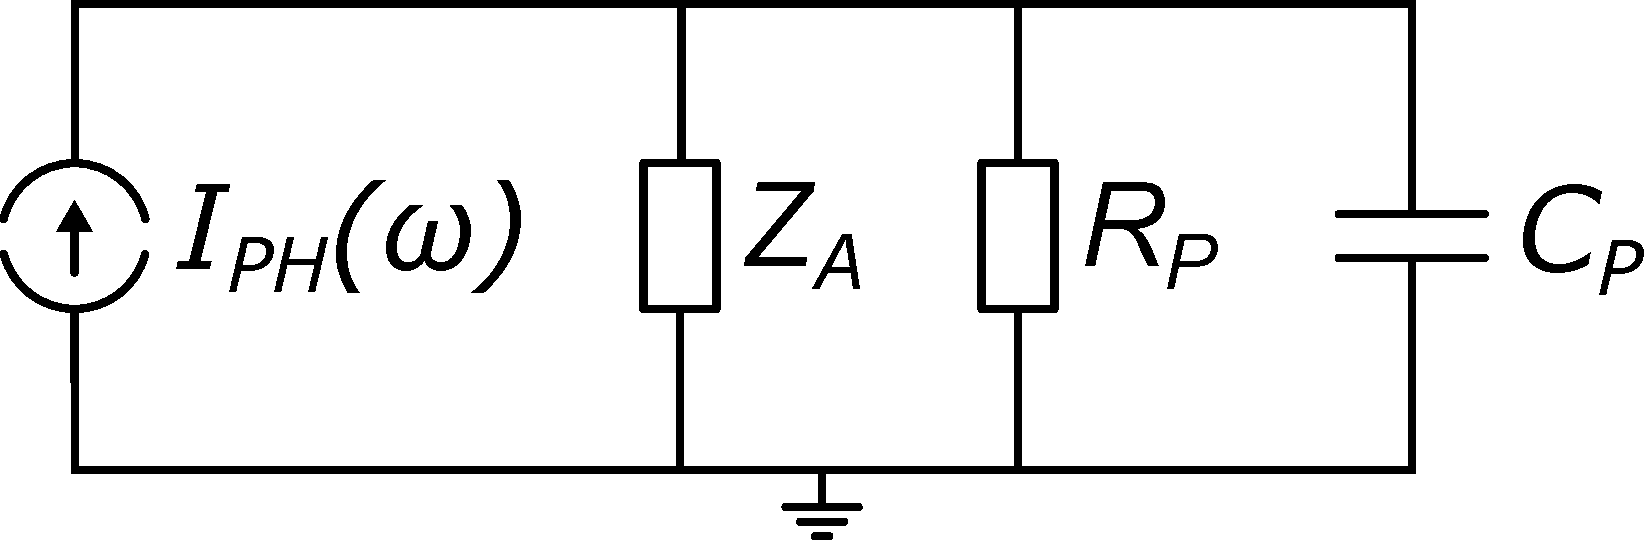
\includegraphics[width=0.7\textwidth]{figures/eq_circuit_PCA.pdf}
	\captionsetup{width=\textwidth}
	\caption{Equivalent circuit for a PCA, consisting of the antenna impedance $Z_A(\omega) = R_A + iB_A(\omega)$, the photoconductive resistance $R_P$ and the photoconductive capacitance $C_P$. The current source $I_{PH}(\omega)$ models the generated photocurrent.}
	\label{PCA_eq}
\end{figure}

Two roll-off factors decrease the emitted THz power at higher frequencies. RC roll-off reflects the influence of the PCAs capacitance and impedance. A PCAs equivalent circuit \cite{fernandezolveraInternationalSystemUnits2019,collinLimitationsTheveninNorton2003} is shown in figure~\ref{PCA_eq}. The current source $I_{PH}(\omega)$ models the radiating element of the antenna. In parallel to the radiating element sits the devices capacitance $C_P$ between the antennas electrodes. The resistance $R_P$ describes the photoconductivity $R_P^{-1} = G_P$ in parallel to the radiation resistance of the antenna $R_A$. Not all energy is radiated, some is stored in the susceptance $B_A(\omega)$. For simplicity, the radiation impedance is modelled as purely ohmic, leaving only $R_A$. Normally $R_{P} \gg R_A$, so the photoconductive resistance can be neglected.  With the made simplifications, the equivalent circuit represents a typical RC circuit in low-pass filter configuration. At higher frequencies, output power is expected to decrease. The current reaching the antenna is reduced by a factor $(1 + i2\pi \nu_{THz}\tau_{RC})^{-1}$, as can be shown by calculating the transfer function of the simplified equivalent circuit: 

\begin{equation}
    H = \frac{Z_{out}}{Z_{in}} = \frac{\frac{1}{i\omega C_P}}{R_A + \frac{1}{i\omega C_P}} = \frac{1}{1 + i\omega R_A C_P} = \frac{1}{1 + i 2\pi \nu_{THz} \tau_{RC}}.    
	\label{transferfunction}
\end{equation}

The factor by which output power will decrease is given by 

\begin{equation}
    \eta_{RC}(\nu_{Thz}) = \frac{1}{1+ (\nu_{THz}/\nu_{RC})^2} = |H|^2,  \qquad  \nu_{RC} = \frac{1}{2\pi\tau_{RC}} = \frac{1}{2\pi R_A C_P},
\end{equation}
where $\nu_{RC}$ is the RC 3 dB frequency.

Not all electron-hole pairs generated by photon absorption contribute to the photocurrent. A portion of charge carriers are trapped and recombine before reaching the electrodes. Due to recombination, the number of available charge carriers for photocurrent generation decreases exponentially over time. From eq. \eqref{eq8}, the average photocurrent over the transit time $\tau_{tr}$ can be calculated, yielding
\begin{align}
	I_{Ph}^{Id}(t) &= \frac{1}{\tau_{rec}} \int_{0}^{\infty} I^{Id}[1 + \cos(\omega_{THz}t + \phi)]e^{\frac{-t}{\tau_{rec}}}dt \notag \\
	I_{Ph}^{Id}(t) &=  I^{Id}\frac{\tau_{rec}}{\tau_{tr}}\left[
		1 + \frac{\sin(\omega_{Thz}t + \phi)}{\sqrt{1 + (\omega_{Thz} \tau_{rec})^2}}
	\right],
\end{align}
where $\tau_{rec}$ is the recombination time. Both the time dependent THZ part and the DC part of the photocurrent are damped due to the trapping of charge carriers by a factor $g = \tau_{rec} /\tau_{tr}$. The factor $g \ll 1$ is called the photoconductive gain. The THz part of the photocurrent is further decreased by the lifetime roll-off 
\begin{equation}
	\eta_{LT}(\omega_{THz}) = \frac{1}{1 + (\omega_{THz}\tau_{rec})^2}.
\end{equation}

In combination with the photoconductive gain $g$ this yields an intrinsic photoconductive roll-off
\begin{equation}
	\eta_{PC}(\omega_{THz}) = g^2\eta_{LT}(\omega_{THz}) = \frac{g^2}{1 + (\omega_{THz}\tau_{rec})^2}.
\end{equation}
Ultimately, the actual THz power emitted by a PCA is given by 

\begin{equation}
    P_{THz}(\omega) = \frac{1}{2}R_A(I_{Ph}^{Id})^2\eta_{ext}^2\eta_{PC}(\omega)\eta_{RC}(\omega).
    \label{eq_power}
\end{equation}

Considering the nonidealities is important for understanding high frequency limitations in THz-TDS setups. This work further evaluates how incorporating resistive elements into the antenna structure affects the mechanisms that limit THz performance. 


\subsection{Photoconductive Antennas for THz-TDS}

\begin{figure}[!]
    \centering
    \begin{minipage}{0.75\textwidth} 
        \centering
        \begin{subfigure}[t]{0.45\textwidth}
            \centering
            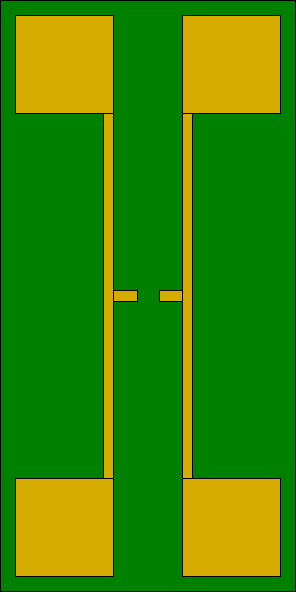
\includegraphics[height=0.32\textheight]{figures/typ_PCA_antenna.pdf}
            \caption{\centering}
            \label{fig:typPCAantenna}
        \end{subfigure}
        \hfill
        \begin{subfigure}[t]{0.45\textwidth}
            \centering
            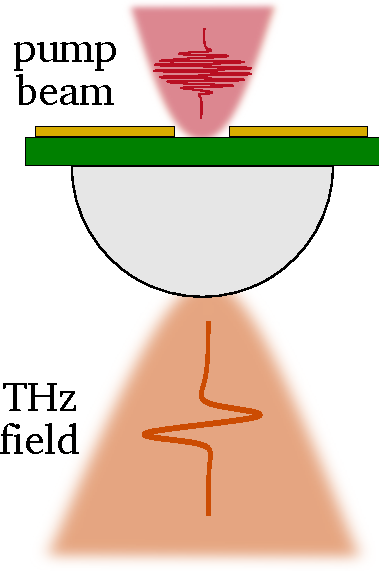
\includegraphics[height=0.32\textheight]{figures/typ_PCA_bias.pdf}
            \caption{\centering}
            \label{fig:typPCAbias}
        \end{subfigure}
        \caption{A typical PCA being used as a receiver in a pulsed system. (a) Typical PCA configuration depicting an H-Dipole antenna with a small active region in between the electrodes. (b) The charge carriers in the active region are optically excited by a femtosecond laser pulse. The device sits on top of a silicon lens. Incoming THz radiation is focused by the lens and biases the antenna.}
        \label{fig:typPCA}
    \end{minipage}
\end{figure}


% The testing of the fabricated devices in this work is limited to the detection of THz radiation. 

% THz antennas based on the photomixing technique usually consist of a small active region sitting in between the antenna's electrodes. For this thesis, the antennas will only be used as recipients for THz radiation. As discussed, PCAs need to be biased externally to emit or detect THz waves. When being used as receivers, the biasing in in PCA is provided by incident THz radiation focused onto the antenna's active region by a hyper-hemispherical silicon lens. A femtosecond laser beam is focused onto the active region as well, creating free electron-hole pairs (see figure~\ref{fig:typPCAbias}).
Figure \ref{fig:typPCA} shows a typical PCA alongside a schematic of its use as a detector in a THz-TDS system. A PCA generally exhibits a radiation resistance $R_A$ in the range of \num{20} - \num{200} \si{\Omega}. The detected THz power and bandwidth depend strongly on the antenna topology. Antenna types commonly used in CW operation, such as logarithmic periodic (log-periodic) antennas \cite{mendisTunableCWTHzSystem2004}, logarithmic spiral (log-spiral) antennas \cite{linRoomtemperatureContinuouswaveTerahertz2025}, or bow-tie antennas \cite{PDFBowtieWideband}, are not equally well suited for pulsed operation. Log-periodic and log-spiral antennas exhibit strong dispersion of THz pulses due to their long arms \cite{fernandezolveraDispersivePropertiesSelfcomplementary2017a}. Because a THz pulse spans multiple frequency components, different spectral parts of the pulse propagate differently within the antenna. Lower-frequency components with longer wavelengths travel more slowly, leading to temporal spreading and pulse distortion. Bow-tie antennas and complementary square spiral antennas \cite{HighPowerGeneration}, by contrast, exhibit lower dispersion and can enhance low-frequency components of the THz spectrum, thereby increasing the dynamic range (DNR).

The most commonly used PCAs in THz-TDS systems are H-Dipole antennas \cite{nandi1550nmDrivenErAs2018} (see Figure \ref{fig:typPCAantenna}) and slotline antennas \cite{kohlhaasPhotoconductiveTerahertzDetectors2019}. Both designs exhibit very low dispersion, which preserves the short duration and integrity of the generated THz pulses. Their  mostly non-dispersive broadband response, combined with a simple geometry, makes them the antennas of choice for many THz-TDS applications. Since this work focuses on improving PCA performance in pulsed operation, slotline antennas will not be discussed further. I-shaped resonant Dipole antennas are introduced as a point of comparison to H-Dipoles. I-shaped dipoles resonate at half the wavelength ($\lambda/2$) of the incident radiation and, like H-Dipoles and slotline antennas, are expected to show little dispersion. They are additionally predicted to provide enhanced sensitivity at lower THz frequencies \cite{nguyenPhotoconductiveDipoleAntennas2017}. I-shaped dipoles serve as a useful benchmark alongside H-Dipoles when evaluating the influence of NiCr modifications on antenna performance

The discussion above has outlined the working principles of PCAs under idealized
assumptions, where the generated photocurrent is directly coupled into free-space radiation. Some nonidealities have been described. Those however are mainly limited to the high-frequency performance of PCAs. This thesis addresses an additional limitation at the low-frequency end of the spectrum: resonances caused by the large metallic pads and antenna feeding structure. These resonances are typically not captured by the model derived above. Understanding these resonances is crucial since they limit the usable bandwidth of photoconductive antennas and motivate the central idea of this work: the introduction of resistive NiCr segments to damp low-frequency resonances. In the following section, the
origin and effects of these pad resonances are analyzed in detail.


\section{Pad Resonances, Effects on TDS}
\begin{itemize}
	\item plot of resonance in low f 
	\item explain why this is bad (FFT, Ringing etc.)
\end{itemize}
\section{Fourier Transform, Ringing}

\chapter{Antenna Design and Simulation}
\section{NiCr Arms to reduce Resonances}
\begin{itemize}
	\item propose NiCr solution to solve pad resonancy problem 
\end{itemize}
\section{Pulsed Antenna Design and Simulation}
Simulations were mainly performed by reusing the simulation file proposed in \cite{nandiErAsInAlGaAsPhotoconductors2021} as a reference for this work. We then replace some part of the original antenna feeding strips by NiCr. The basic simulation steps will be outlined as a short review of \cite{nandiErAsInAlGaAsPhotoconductors2021}.   

\subsection{Reference Antenna Topology}

\begin{figure}
    \centering
    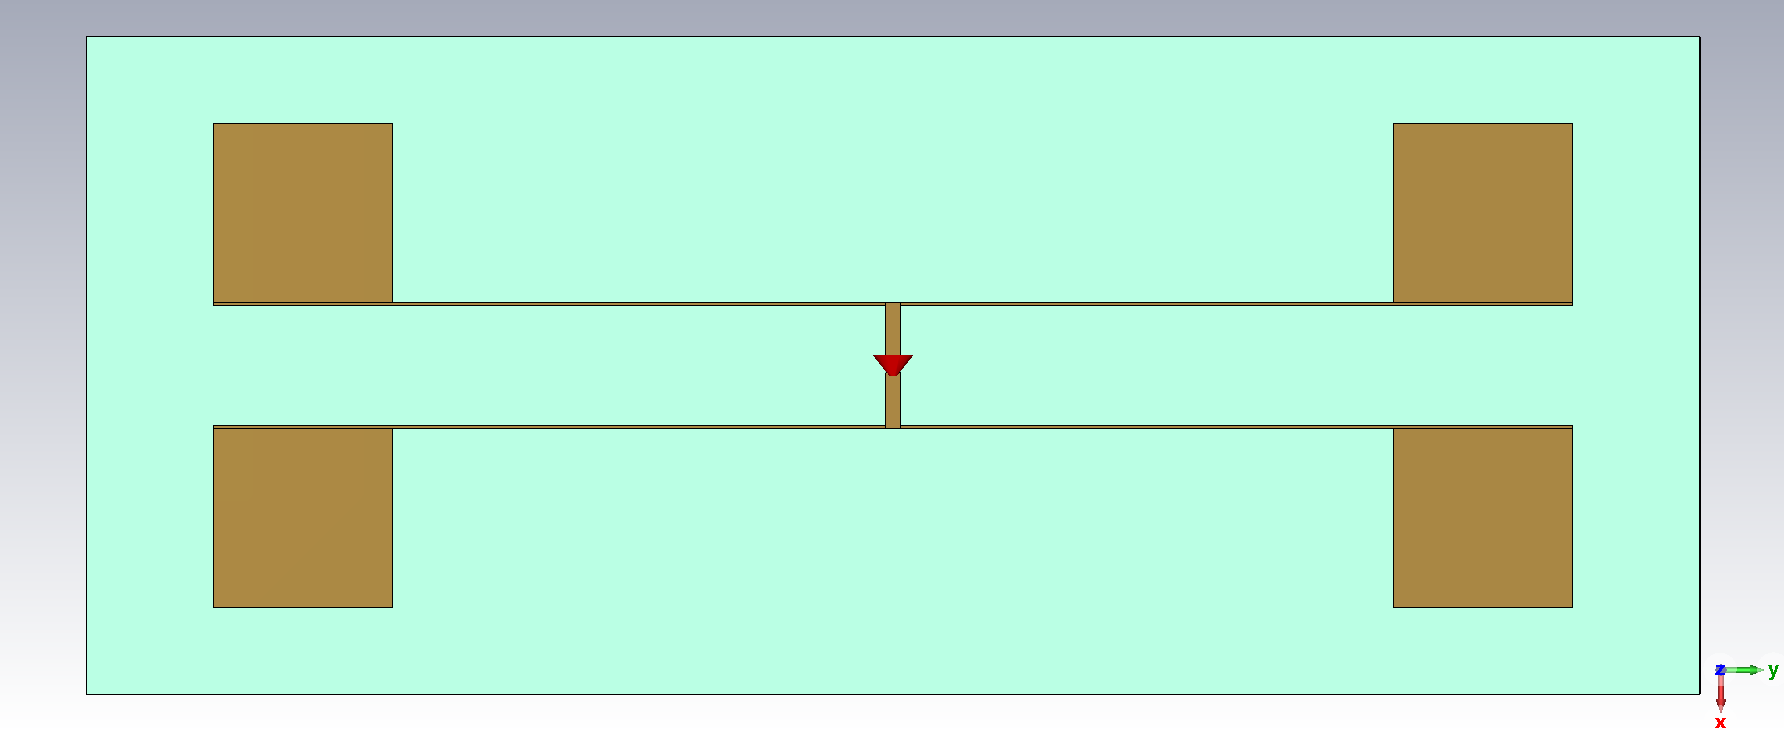
\includegraphics[width=\linewidth]{figures/H_Dipole_ref.png}
    \caption{H-Dipole PCA used as reference for simulations in CST Studio Suite. The antennas golden structure sits on top of the green substrate. In between the electrodes sits the lumped element port.}
    \label{ref_h_dipole_for_sim}
\end{figure}

The H-Dipole antennas are deposited on the active photoconducting material ($\sim$ \num{1.5} \si{\micro\meter}). Below the active material sits a semi-insulating InP substrate ($\sim$ \num{500} \si{\micro\meter}). Additionally, a hyper-hemispherical silicon lense with a radius of \num{6.1} \si{\milli\meter} is attached to the substrate for efficient out-coupling of the generated THz signal. Simulating the entire structure including the silicon lense would not be feasible as too much computational power would be needed. The simulation is simplified by using a technique described in  ref. \cite{llombartTHzTimeDomainSensing2012,garufoNortonEquivalentCircuit2018}. The antenna is positioned at the air–substrate interface, where the \enquote{open add space} boundary condition is applied in CST. All other boundaries use the \enquote{open} condition, which absorbs electromagnetic radiation and mimics an infinitely extended medium. Figure \ref{ref_h_dipole_for_sim} shows the topology of the reference antenna structure used in the simulation. The substrate thickness is set to at least one wavelength across all relevant frequencies. A lumped element port is used to excite the on-substrate H-dipole antenna. For reliable results, the port dimensions should be at least five times smaller than the effective wavelength. As we only investigate THz performance up to \num{1} \si{\tera\hertz}, this criterion should always be fulfilled. 

\subsection{NiCr-Induced Antenna Topology}
The reference antenna topology is used to evaluate the THz performance of NiCr-induced feeding strips. Additionally to the described topology, NiCr properties are added. We start by defining NiCr's material properties. NiCr is defined as 

\textbf{TODO: properties aus CST adden}.

In the reference H-Dipole topology, the deposited metal is defined as perfectly electrically conducting (PEC). This is good enough for simulation purposes as gold can be approximated as a perfect conductor of electricity. Some part of the PEC in the antenna feeding strip is now replaced by NiCr. We start inducing the NiCr at the antenna's electrodes. This means that the longer the NiCr-strip, the closer it is to the antenna's pads. Figure (\textbf{TODO: Figure für NiCr Antenna Sim}) shows an example for a H-Dipole antenna where some part of it's feeding structure is replaced by NiCr. 



\subsection{Geometries to be simulated}
The length $l_{NiCr}$ of the NiCr strip defines its resistance, as $R_{NiCr} \propto l_{NiCr}$. This is why multiple configurations have to be simulated to choose appropriate lengths for processing. 

\begin{figure}[ht]
    \centering
    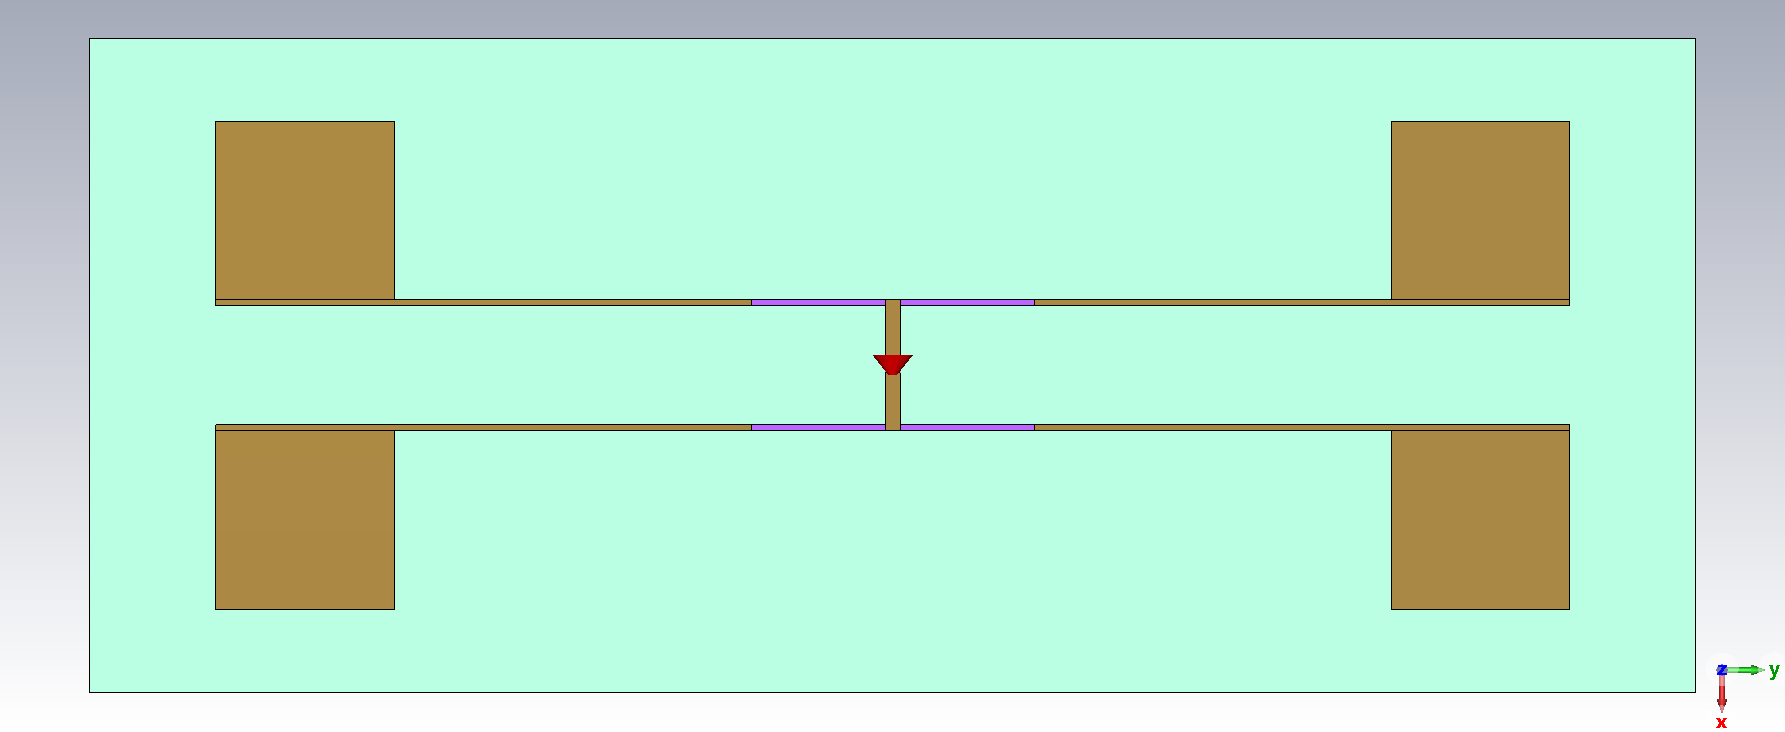
\includegraphics[width=\linewidth]{figures/H_Dipole_NiCr copy.png}
    \caption{H-Dipole PCA including a NiCr-section (purple). The antennas golden structure sits on top of the green substrate. In between the electrodes sits the lumped element port.}
    \label{ref_h_dipole_for_sim}
\end{figure}




\section{Simulation Results}
Intro Sentence!!

The distribution of the surface current is a measure of the electromagnetic wave's propagation through the antenna structure. Using the surface current distribution we can calculate the THz field emitted by the antenna using Maxwell's equations. Low frequency resonances caused by the large pad sizes are to be reduced. We present the surface current distribution in four H-Dipole antennas with differing NiCr-sections. The four configurations are compared at two distinct frequencies: \num{100} \si{\giga \hertz} (see figure \ref{sc_100ghz_comp}) and \num{1} \si{\tera \hertz}. The simulations at \num{100} \si{\giga \hertz} show that adding a NiCr-section to the antenna feed should reduce the low frequency surface current spikes caused by the antenna feeds and pads.


\begin{figure}[ht]
    \centering
    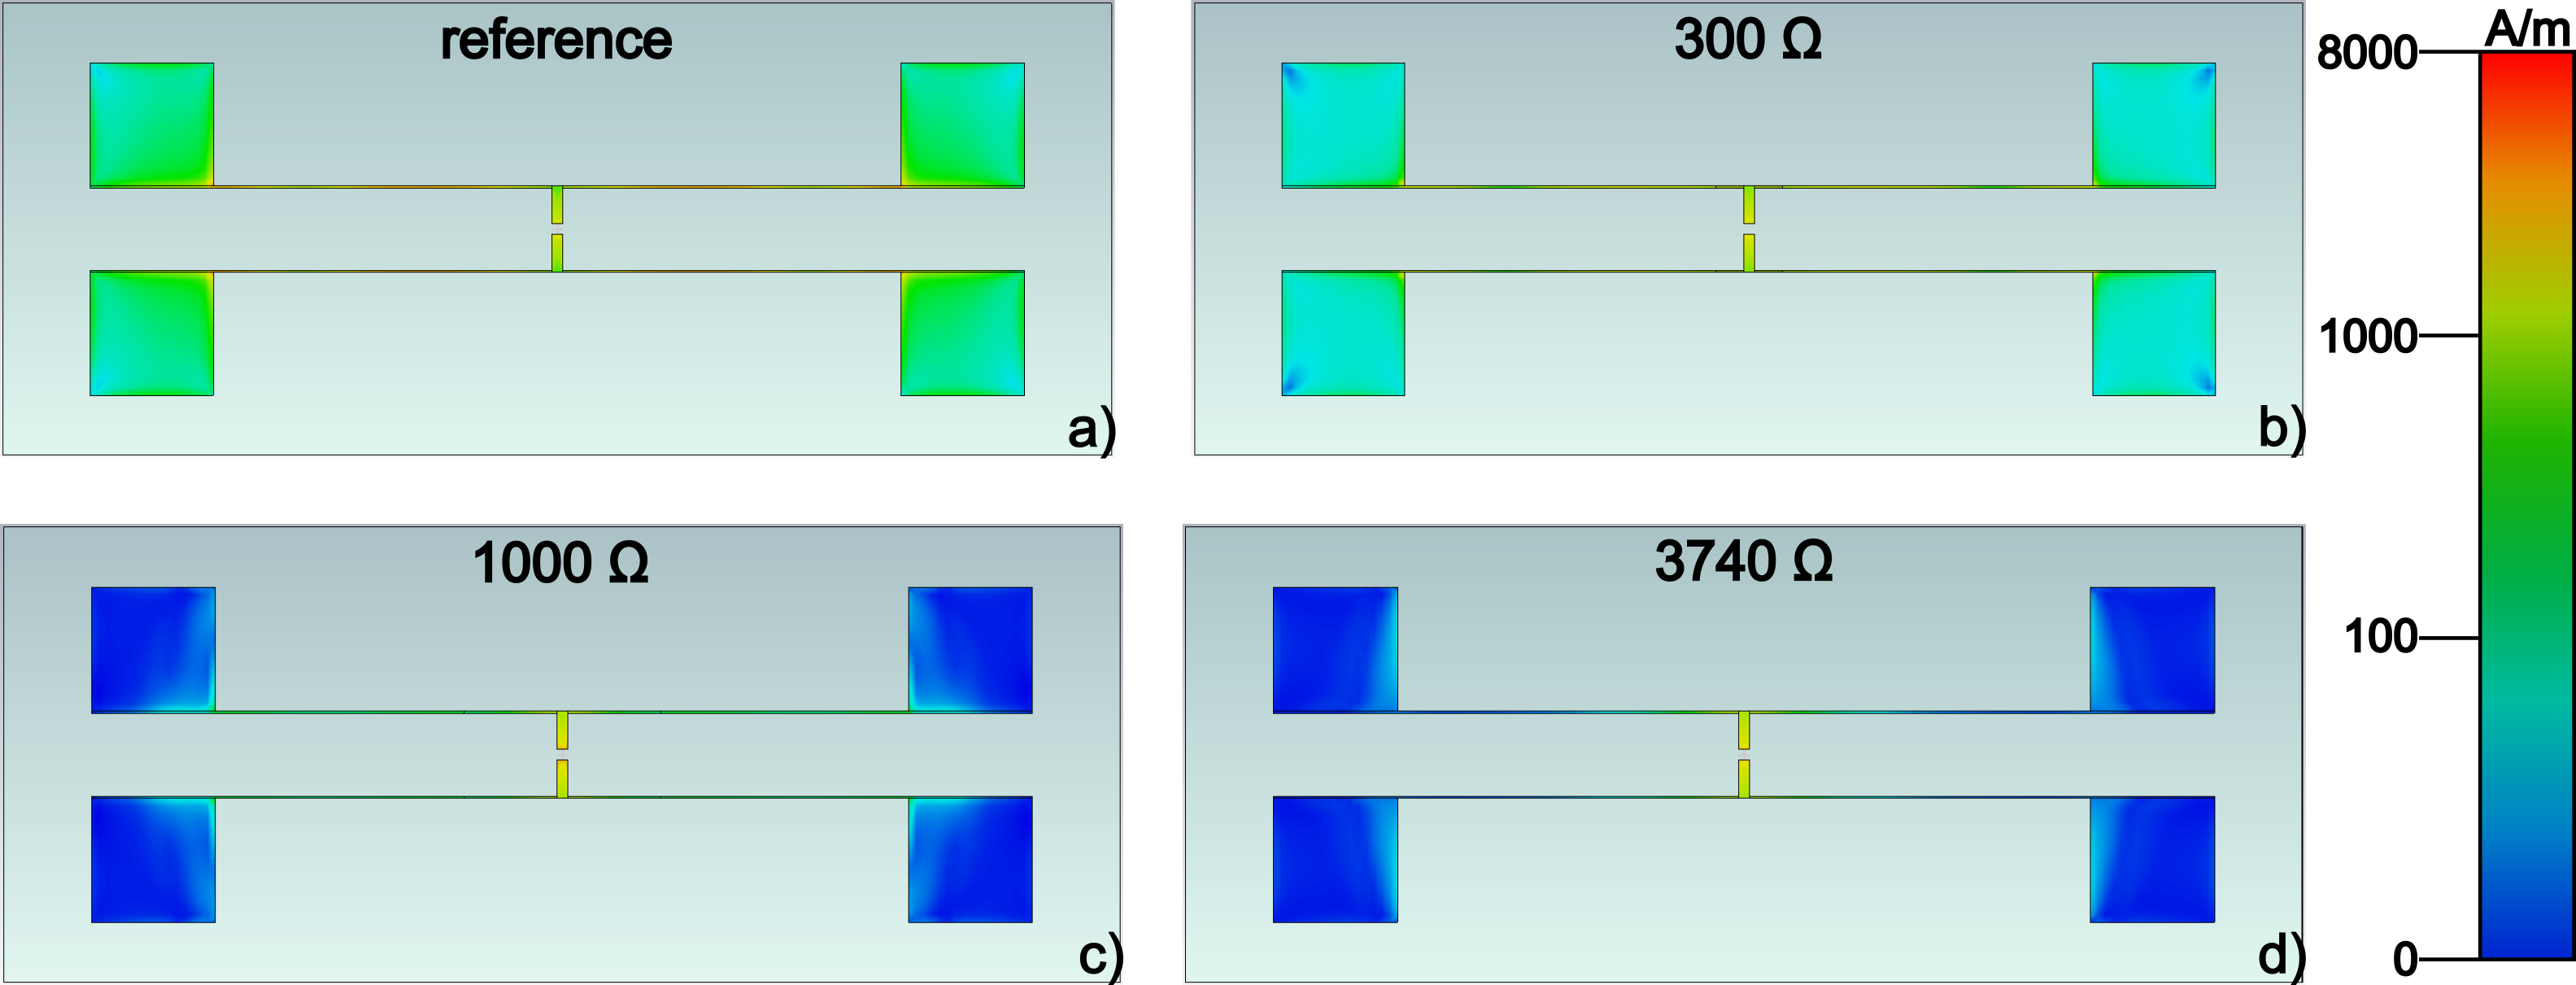
\includegraphics[width=\linewidth]{figures/Contour_Plots_v2/100Ghz_SC_sim_plots.png}
    \caption{Contour plots of the simulated surface currents at \num{100} \si{\giga \hertz} for four different H-Dipole antenna configurations. The surface current is plotted logarithmically. a) Surface current distribution in the reference H-Dipole. b) Surface current distribution with the NiCr-section corresponding to a resistance of $R_{NiCr} = 300$ \si{\ohm}. c) Surface current distribution with the NiCr-section corresponding to a resistance of $R_{NiCr} = 1000$ \si{\ohm}. d) Surface current distribution with the NiCr-section corresponding to a resistance of $R_{NiCr} = 3740$ \si{\ohm}.}
    \label{sc_100ghz_comp}
\end{figure}

Figure \ref{sc_100ghz_comp} a) depicts the surface current in the reference H-Dipole antenna where no NiCr is added. A fairly even distribution of the surface current along the antenna structure can be observed. Red sections along the antenna's feeding strip indicate that a high extend of the THz radiation is emitted in the strip, indicating the leaky-wave behavior of the antenna at low frequencies. Low-frequency harmonics are caused by these resonances along the feeding strip. We also see that the surface current distribution in the electrodes and the pads is fairly similar at surface currents of a few 100 A$/$m, causing the high low frequency resonances. 

A NiCr-section equivalent to a resistance of $R_{NiCr} = 300$ \si{\ohm} is added to the reference H-Dipole in figure \ref{sc_100ghz_comp} b). Already we can observe a concentration of the surface current around the antenna's electrodes. The surface current distribution in the pads now only reaches values of a few 10 A$/$m. Low frequency pad resonances still occur but are damped in a,amplitude. Along the feeding strips, resonant spots are observable, indicating that low frequency harmonics are still present. 


At $R_{NiCr} = 1000$ \si{\ohm} (see figure \ref{sc_100ghz_comp} c), the surface current is heavily concentrated around the antenna's electrodes. The surface current distribution in the pads nearly drops to zero. The surface current along the feeding strip appears relatively homogenous, indicating an absence of leaky-wave modes along the axis parallel to the strip and thus a reduction of low frequency time-harmonics. This is the non-resonant low frequency behavior we want to achieve. $R_{NiCr} = 3740$ \si{\ohm} (see figure \ref{sc_100ghz_comp} d)) is the maximum resistance we can achieve. A very similar surface current distribution compared to figure \ref{sc_100ghz_comp} c) is observable. The surface current along the feeding strip is further reduced and continues to concentrate around the electrodes. 

\begin{figure}[ht]
    \centering
    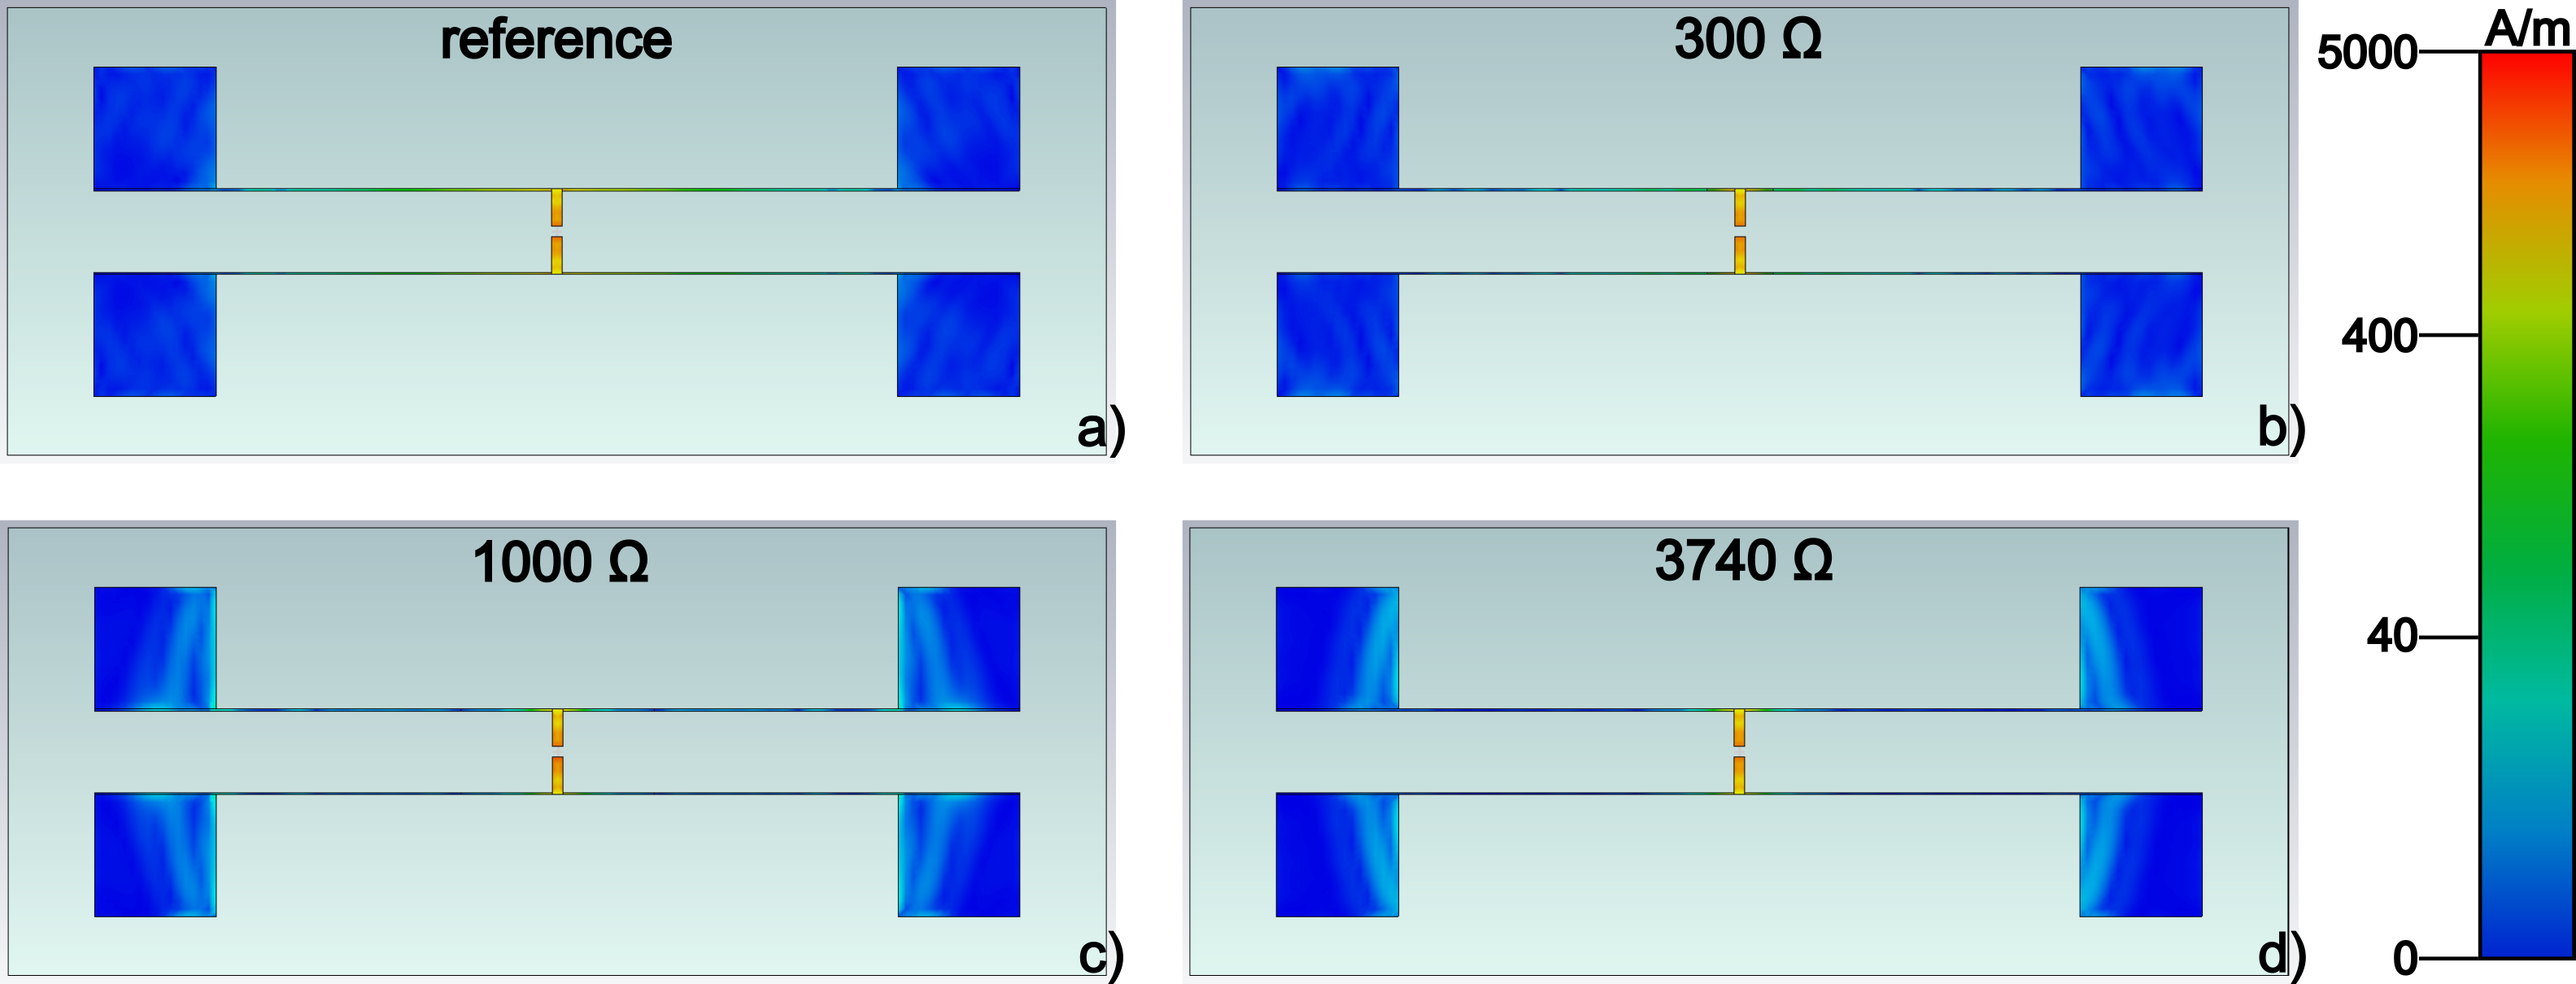
\includegraphics[width=\linewidth]{figures/Contour_Plots_v2/1Thz_SC_sim_plots.png}
    \caption{Contour plots of the simulated surface currents at \num{1} \si{\tera \hertz} for four different H-Dipole antenna configurations. The surface current is plotted logarithmically. a) Surface current distribution in the reference H-Dipole. b) Surface current distribution with the NiCr-section corresponding to a resistance of $R_{NiCr} = 300$ \si{\ohm}. c) Surface current distribution with the NiCr-section corresponding to a resistance of $R_{NiCr} = 1000$ \si{\ohm}. d) Surface current distribution with the NiCr-section corresponding to a resistance of $R_{NiCr} = 3740$ \si{\ohm}.}
    \label{sc_1thz_comp}
\end{figure}

It is important that adding the NiCr-section only affects the surface current generated at lower frequencies. At higher frequencies ($\nu > 100$ \si{\giga \hertz}), the coupling of THz radiation into the antenna is expected to occur predominantly at the electrodes due to the decreasing wavelength. Ideally, the NiCr segments should exert minimal influence on the surface currents propagating from the electrodes to the antenna pads. Figure \ref{sc_1thz_comp} shows the simulated surface current distribution at \num{1} \si{\tera \hertz} in the four antenna configurations which were already discussed at \num{100} \si{\giga \hertz}. 

At \num{1} \si{\tera \hertz}, the surface current distribution appears largely invariant across different antenna configurations. This antenna behavior is intended. The incorporation of NiCr segments introduces a resistive component that attenuates surface currents at lower frequencies. At higher frequencies, the surface current is able to propagate despite the added resistance. 







\chapter{Device Fabrication and DC Characterization}
\begin{itemize}
	\item we grew ErInGas oder so (nur kurz erwähnen, nicht Teil der Arbeit)
	\item maybe talk about typical features we would expect 
\end{itemize}


\section{Device Fabrication Process}
The device fabrication consists of three main processes. Included in these processes are various litography steps, evaporation of different metals, wet etching and deposition of silicon nitride as an anti-reflective coating. First, the desired antenna structure is imprinted on our wafer through contact litogrpahy and the antennas metal is deposited. Then, mesa litography and mesa etching is applied. In the end, an antireflective coating is deposited. 

\subsection{Antenna Structure Litography and Metal Deposition}

\textbf{TODO: ABBILDUNG}

A litography mask is fabricated containing the desired antenna structures. A \num{7} $\times$ \num{8} \si{\milli\meter} sample of the ErAs:In(Al)GaAs photoconductor, grown on a \num{500} \si{\micro\meter} InP:Fe substrate wafer is cleaved out from the wafer. The desired antenna structures are imprented onto the sample via contact litography. Structures as small as approximately \num{1} \si{\micro\meter} are desired, so good contact is critical in this process. 

A thin layer of AZ 5414E image reversal photoresist is deposited on the sample. By spin coating the sample with photoresist, a uniform layer is achieved. The sample is then developed using AZ MIF 726, leaving a \num{6} $\times$ \num{7} \si{\milli\meter} of photoresist. This helps in having good contact when applying contact litography steps.

The image reversal effect of AZ 5414E is achieved by baking the sample at \num{120} \si{\celsius} for one minute and exposing it to ultraviolet light of five times the initial exposure time. The AZ 5415E is transformed from positive to negative. A second litographic step is performed leaving the actual antenna structures exosed. 

Before depositing the metal for the PCAs, the samples are dipped into a 1:1 solution of H\textsubscript{2}O and HCl for \num{30} seconds to remove the oxide layer which forms at the surface. This step greatly improves the adhesion of the deposited metal. The antenna electrodes and contact pads are fabricated by depositing a \num{180} \si{\nano\meter} layer of gold (Au) on top of a \num{20} \si{\nano\meter} layer of Chrome (Cr) via electron beam evaporation. The Cr-layer improves the contact with the semiconducting material. The antenna feeds are fabricated by combining the deposition of an Au-layer on top of a Cr-layer and a nichrome (NiCr) layer. The two layers are joined.  

\textbf{TODO: maybe further explain how NiCr is deposited}

After completing the metal deposition step, the sample is dipped in acetone. This way we get rid of the unwanted metal on our sample. 

An additional annealing step is needed after metal deposition to further improve the metal-semiconductor-contact. Such an annealing process reduces the interface impurities and creates good contact on the atomic scale between the metal and the semiconducting material \cite{tahamtanInvestigationEffectAnnealing2011}. Annealing is performed at a temperature of \num{425} \si{\celsius} for \num{30} seconds. After annealing, the antennas IV-characteristics are measured to ensure ohmic contacts. 

\subsection{Mesa Litography and Mesa Etching}

A thick layer of AZ 1518 HS photoresist is deposited onto the sample. Again, spin scoating ensures a uniform photoresistive layer. This step is followed by hard baking the sample covered by photoresist at \num{110} \si{\celsius} for \num{15} minutes. The hard baking makes the residual solvent present in the resist evaporate, stabilizes the printed structure and improves the bond between the resist and the material. 

The thin ErAs:In(Al)GaAs photocondutive material is etched from the areas that were not protected by the photoresist layer using 
hydrogen peroxide (H\textsubscript{2}O\textsubscript{2}), sulphuric acid (H\textsubscript{2}SO\textsubscript{4}) and water mixed in appropriate proportion. The semi-insulating InP:Fe substrate is left exposed in those areas. 

By mesa etching, the active InGaAs layer is removed from the entire sample except between the electrodes and under the antenna and pads. This process ensures a high resistance is with a minimal dark current. A minimal dark current drastically improves the signal-to-noise ratio of the THz signal. 

\textbf{TODO: ABBILDUNG}

\subsection{Anti-Reflection Coating Deposition}
An anti-reflection coating (ARC) is deposited above the active region. The ARC layer helps improving the transmission of the THz by minimizing reflection \cite{chenAntireflectionImplementationsTerahertz2014} and protects the device from external damage. The ARC is fabricated by growing a silicon nitride (Si\textsubscript{3}N\textsubscript{4}) layer on top of the sample via plasma-enhanced chemical vapor deposition. 

After depositing the ARC, another thick layer of AZ 1518 HS photoresist is deposited on the sample to form the required shapes of the ARC over the mesa. The photoresist only covers the antennas electrode structure. 

The Si\textsubscript{3}N\textsubscript{4} is etched out from the unprotected areas, exposing the contacting metal pads attached to the antenna. The etching is done in a plasma etching machine using carbon tetra-fluoride (CF\textsubscript{4}) as the etching agent. After etching of Si\textsubscript{3}N\textsubscript{4} the photoresist is removed by dipping the sample into acetone.


\textbf{TODO: ABBILDUNG maybe}
\section{DC Characterization ??}

\chapter{Experimental Setup}
\section{THz TDS setup}
\section{Alignment ??}
\section{Data Analysis ??}

\chapter{Results and Discussion}

\chapter{Summary and Outlook}

\printbibliography

\end{document}
